\chapter{Fe-Ru Potential}
\label{chapter:appendix-ferupotential}

This potential has been developed specifically for Fe and Ru where the atoms are in an \acrshort{fcc} structure.  Particular weighting was given to the relaxed configurations of each pure element, those with small additions of Ru to Fe and surface/slab configurations.

\section{Tabulated Potential}

The files for the potential are large, with the \acrshort{lammps} version being over 7,000 lines long containing 35,000+ data points.  They are not included here but are available to download from:

https://github.com/BenPalmer1983/fepd\_feru\_potential



\clearpage
\FloatBarrier
\section{Potential Function Plots}

The seven functions that make up the potential are plotted in figure \ref{fig:feru-fcc-function-plots}.

\begin{figure}[htb]
\begin{subfigure}{.32\textwidth}
  \centering
  \includegraphics[width=.94\linewidth]{chapters/potentials_fe_pd_ru/feru_potential/function_plots/fefe_pair.eps}  
  \caption{Fe-Fe Pair}
  \label{fig:feru-fefe-pair}
\end{subfigure}
\begin{subfigure}{.32\textwidth}
  \centering
  \includegraphics[width=.94\linewidth]{chapters/potentials_fe_pd_ru/feru_potential/function_plots/feru_pair.eps}  
  \caption{Fe-Ru Pair}
  \label{fig:feru-feru-pair}
\end{subfigure}
\begin{subfigure}{.32\textwidth}
  \centering
  \includegraphics[width=.94\linewidth]{chapters/potentials_fe_pd_ru/feru_potential/function_plots/ruru_pair.eps}  
  \caption{Ru Ru Pair}
  \label{fig:feru-ruru-pair}
\end{subfigure}
\begin{subfigure}{.32\textwidth}
  \centering
  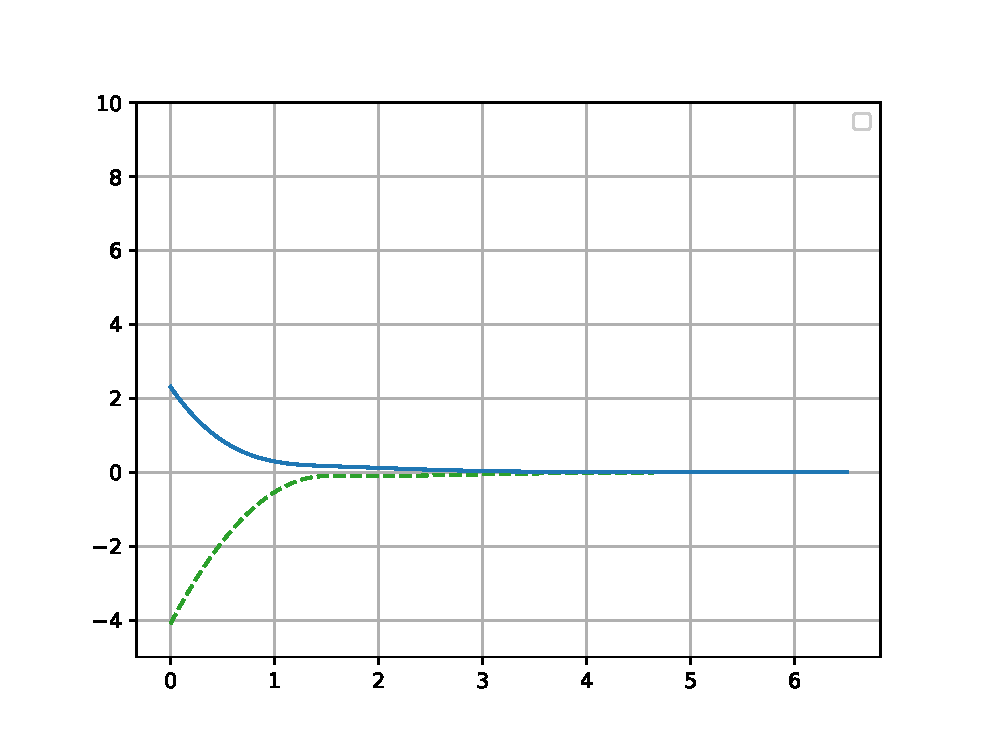
\includegraphics[width=.94\linewidth]{chapters/potentials_fe_pd_ru/feru_potential/function_plots/fe_dens.eps}  
  \caption{Fe Density}
  \label{fig:feru-fe-dens}
\end{subfigure}
\begin{subfigure}{.32\textwidth}
  \centering
  \includegraphics[width=.94\linewidth]{chapters/potentials_fe_pd_ru/feru_potential/function_plots/fe_embe.eps}  
  \caption{Fe Embed}
  \label{fig:feru-fe-embe}
\end{subfigure}
\begin{subfigure}{.32\textwidth}
  \centering
  \includegraphics[width=.94\linewidth]{chapters/potentials_fe_pd_ru/feru_potential/function_plots/ru_dens.eps}  
  \caption{Ru Density}
  \label{fig:feru-ru-dens}
\end{subfigure}
\begin{subfigure}{.32\textwidth}
  \centering
  \includegraphics[width=.94\linewidth]{chapters/potentials_fe_pd_ru/feru_potential/function_plots/ru_embe.eps}  
  \caption{Ru Embed}
  \label{fig:feru-ru-embe}
\end{subfigure}
\label{fig:fepd-fcc-function-plots}
\caption{Binary Alloy Potential for Fe-Ru}
\end{figure}









\clearpage
\section{Potential vs DFT}

The potentials were derived with a larger weight applied to a smaller set of configurations.  How well the potential fits to the \acrshort{dft} results in terms of energy is given in figure \ref{fig:feru-energy-fit}.

\begin{figure}[htb]
\begin{subfigure}{.42\textwidth}
  \centering
  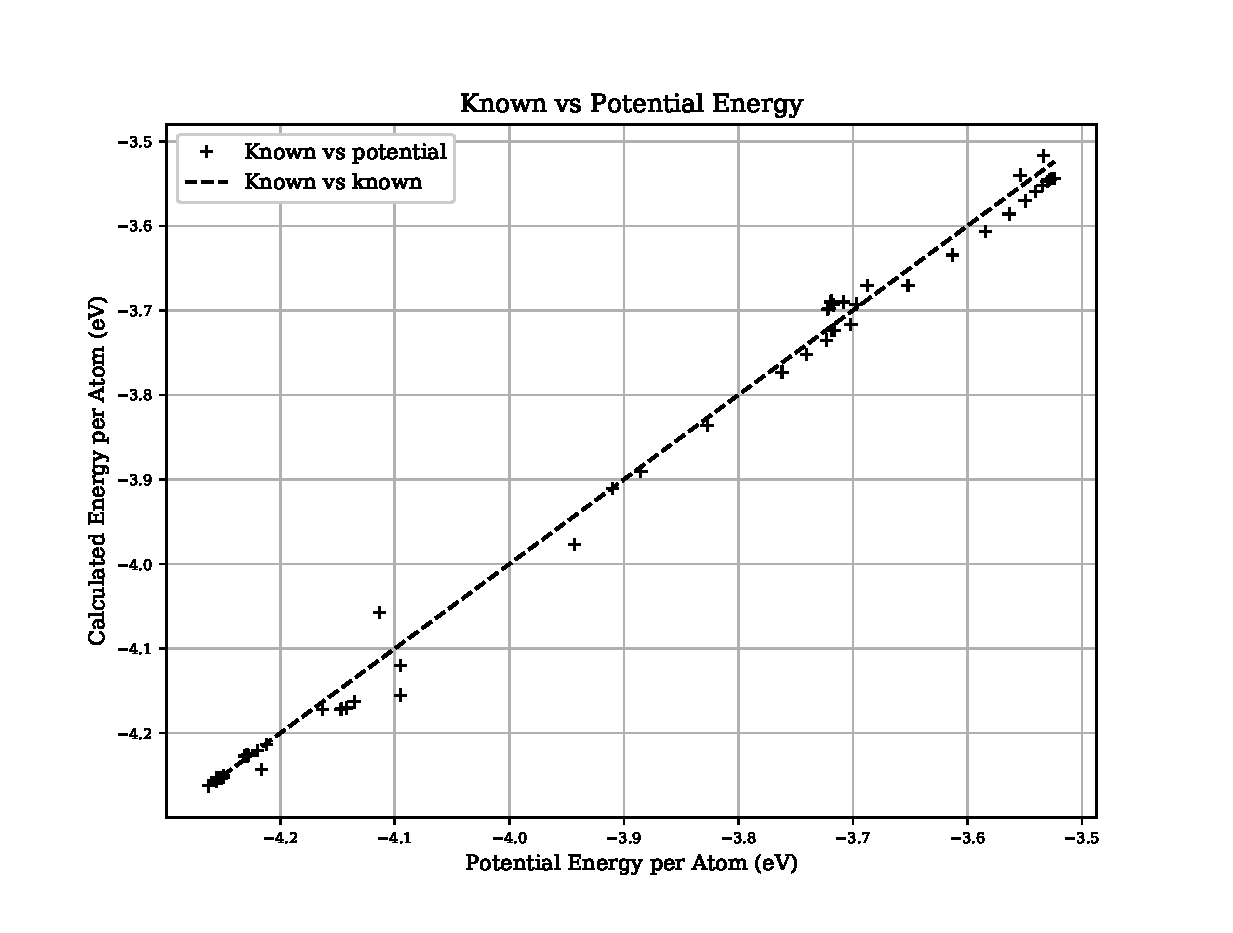
\includegraphics[width=.94\linewidth]{chapters/potentials_fe_pd_ru/feru_potential/potential_known_energy_fit_set.eps}  
  \caption{DFT vs Potential, highly weighted configurations}
  \label{fig:feru-energy-fit}
\end{subfigure}
\begin{subfigure}{.42\textwidth}
  \centering
  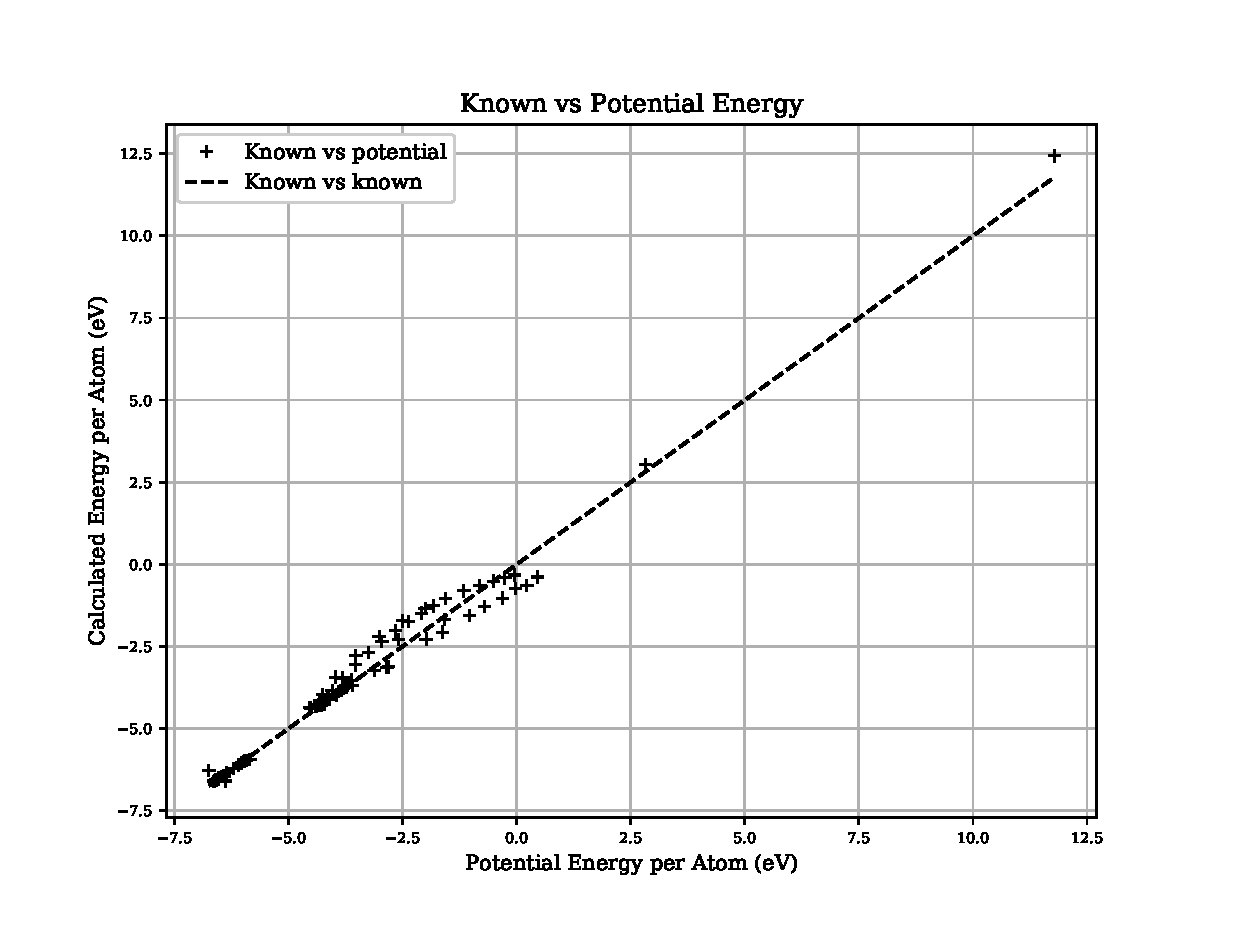
\includegraphics[width=.94\linewidth]{chapters/potentials_fe_pd_ru/feru_potential/potential_known_energy_full_set.eps}  
  \caption{DFT vs Potential, all configurations}
  \label{fig:feru-energy-full}
\end{subfigure}
\label{fig:feru-energy-fit}
\end{figure}

The \acrshort{dft} computed surface energy, as the slab forms from the increased gap between two surfaces, is given in figure \ref{fig:feru-energy-fitting}.

\begin{figure}[htb]
\begin{subfigure}{.42\textwidth}
  \centering
  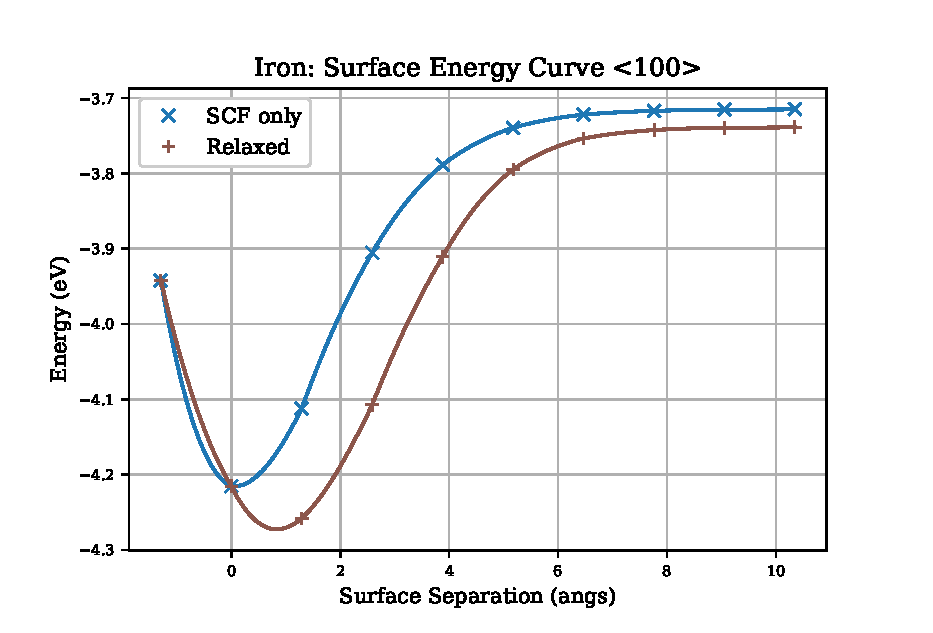
\includegraphics[width=.94\linewidth]{chapters/potentials_fe_pd_ru/feru_potential/fe_surface_energy.eps}  
  \caption{Fe surface energy at a range of surface separations}
  \label{fig:fepd-fefcc-rose}
\end{subfigure}
\begin{subfigure}{.42\textwidth}
  \centering
  \includegraphics[width=.94\linewidth]{chapters/potentials_fe_pd_ru/feru_potential/ru_surface_energy.eps}  
  \caption{Ru surface energy at a range of surface separations}
  \label{fig:feru-fefcc-bmeos}
\end{subfigure}
\label{fig:feru-energy-fitting}
\caption{Equation of State plots from this potential for \acrshort{fcc} Fe}
\end{figure}











\clearpage
\section{Bulk Properties}

%%%%%%%%%%%%%%%%%%%%%%%%%%%%%%%%%%%%%%%%%%%%%%%%%%%%%%%%%%%%%%%%%%%%%%
%  Iron FCC Bulk Properties
%%%%%%%%%%%%%%%%%%%%%%%%%%%%%%%%%%%%%%%%%%%%%%%%%%%%%%%%%%%%%%%%%%%%%%

\FloatBarrier
\subsection{Iron FCC}

\subsubsection{Bulk Property Values}


\begin{table}[ht]
\renewcommand{\arraystretch}{1.2}
\centering
\resizebox{\columnwidth}{!}{%
\begin{tabular}{lcccccc}
\hline\hline
Property & \multicolumn{3}{c}{DFT Computed} & \multicolumn{3}{c}{This Potential} \\
\hline\hline
$a_0$ (angs)         & \multicolumn{3}{c}{3.42}   & \multicolumn{3}{c}{3.42} \\
Basis            & \multicolumn{3}{c}{$\begin{bmatrix} 1.0 & 0.0 & 0.0 \\ 0.0 & 1.05 & 0.0 \\ 0.0 & 0.0 & 1.0  \end{bmatrix}$} & \multicolumn{3}{c}{$\begin{bmatrix} 1.0 & 0.0 & 0.0 \\ 0.0 & 1.05 & 0.0 \\ 0.0 & 0.0 & 1.0  \end{bmatrix}$} \\
$E_{coh}$ (eV)           & \multicolumn{3}{c}{-4.26}  & \multicolumn{3}{c}{-4.27} \\
$B_0$ (GPa)              & \multicolumn{3}{c}{226.1(a) 222.0(b)}  & \multicolumn{3}{c}{246.6(a) 235.2(b)} \\
Stiff.1 (GPa) & \multicolumn{3}{c}{$\begin{bmatrix} 364.6 & 141.6 & 233.8 & 0 & 0 & 0 \\ 141.6 & 298.7 & 130.40 & 0 & 0 & 0 \\ 233.8 & 130.4 & 364.6 & 0 & 0 & 0 \\ 0 & 0 & 0 & 186.3 & 0 & 0 \\ 0 & 0 & 0 & 0 & 266.8 & 0 \\ 0 & 0 & 0 & 0 & 0 & 186.3 \end{bmatrix}$}   & \multicolumn{3}{c}{$\begin{bmatrix} 312.6 &  182.3 & 222.8 & 0 & 0 & 0 \\ 182.3 & 321.6 & 182.3 & 0 & 0 & 0 \\ 222.8 & 182.3 & 312.6 & 0 & 0 & 0 \\ 0 & 0 & 0 & 171.9 & 0 & 0 \\ 0 & 0 & 0 & 0 & 223.1 & 0 \\ 0 & 0 & 0 & 0 & 0 & 171.9 \end{bmatrix}$} \\
Stiff.2 (GPa) & \multicolumn{3}{c}{}   & \multicolumn{3}{c}{$\begin{bmatrix} 329.3 & 205.3 & 205.3 & 0 & 0 & 0 \\ 205.3 & 329.3 & 205.3 & 0 & 0 & 0 \\ 205.3 & 205.3 & 329.3 & 0 & 0 & 0 \\ 0 & 0 & 0 & 198.4 & 0 & 0 \\ 0 & 0 & 0 & 0 & 198.4 & 0 \\ 0 & 0 & 0 & 0 & 0 & 198.4 \end{bmatrix}$} \\
\hline\hline
\end{tabular}%
}
\caption{The lattice parameter, cohesive energy and bulk modulus were determined by fitting the Birch-Murnaghan equation of state.  The bulk modulus is computed from the Birch-Murnaghan equation of state (a) and the average Reuss and Voight Bulk Moduldus (b). The elastic constants computed for the potential in stiffness (1) were computed using the method by Ravindran et al\cite{dfttisiravindran} and in stiffness (2) by Mehl et al\cite{mehlsp}\cite{elasticpropertiesmehl}.}
\end{table}


\subsubsection{Equation of State Plots}

Both the Birch-Murnaghan and Rose-Vinet equation of states are used in the fitting process.

\begin{figure}[htb]
\begin{subfigure}{.44\textwidth}
  \centering
  \includegraphics[width=.94\linewidth]{chapters/potentials_fe_pd_ru/feru_potential/eos/rose_plot_bp_1.eps}  
  \caption{Rose-Vinet}
  \label{fig:feru-fefcc-rose}
\end{subfigure}
\begin{subfigure}{.44\textwidth}
  \centering
  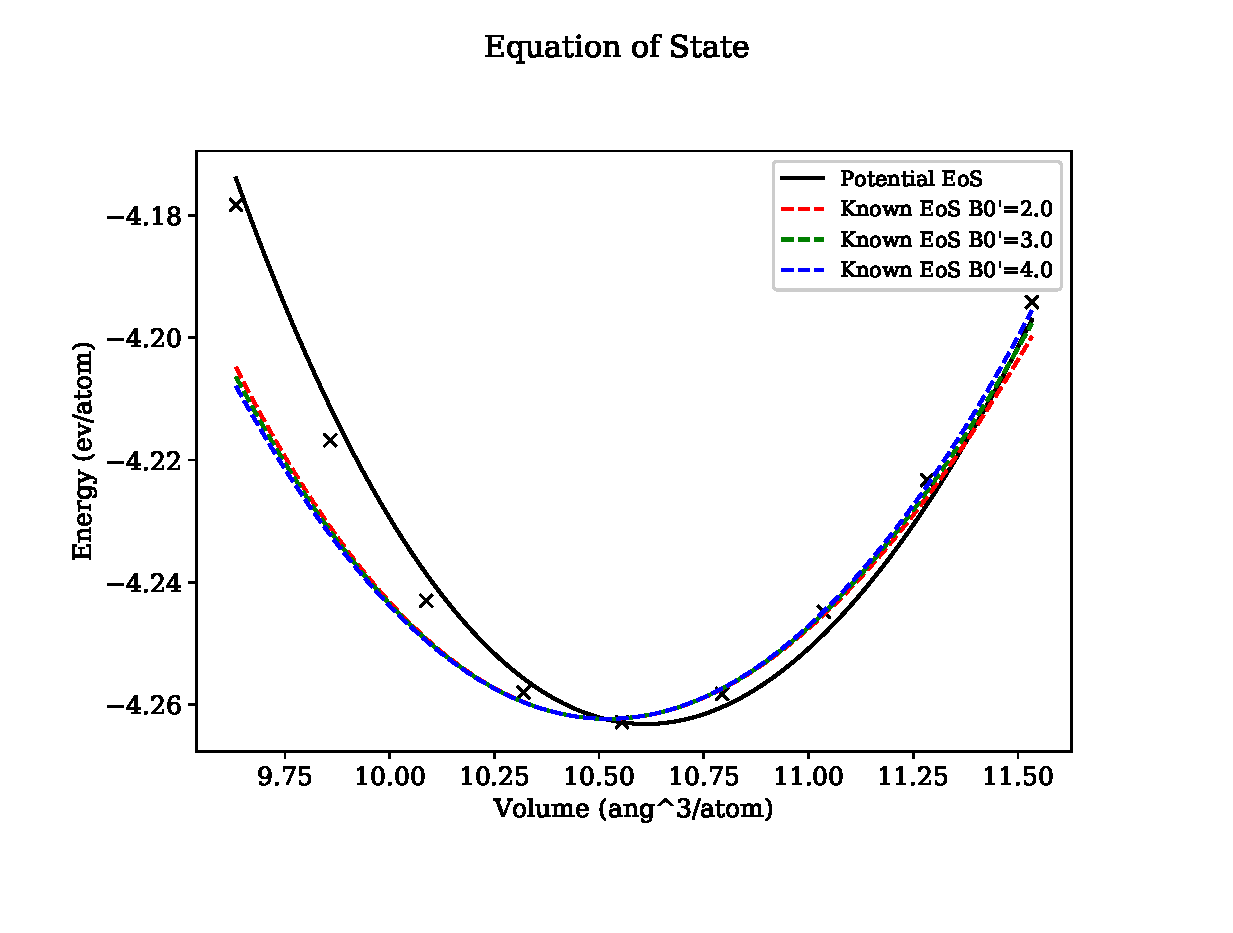
\includegraphics[width=.94\linewidth]{chapters/potentials_fe_pd_ru/feru_potential/eos/equation_of_state_bp_1.eps}  
  \caption{Birch Murnaghan}
  \label{fig:feru-fefcc-bmeos}
\end{subfigure}
\label{fig:feru-fefcc-equation-of-state}
\caption{Equation of State plots from this potential for \acrshort{fcc} Fe}
\end{figure}


\clearpage
\subsubsection{Elastic Constant Plots}

\begin{figure}[htb]
\centering
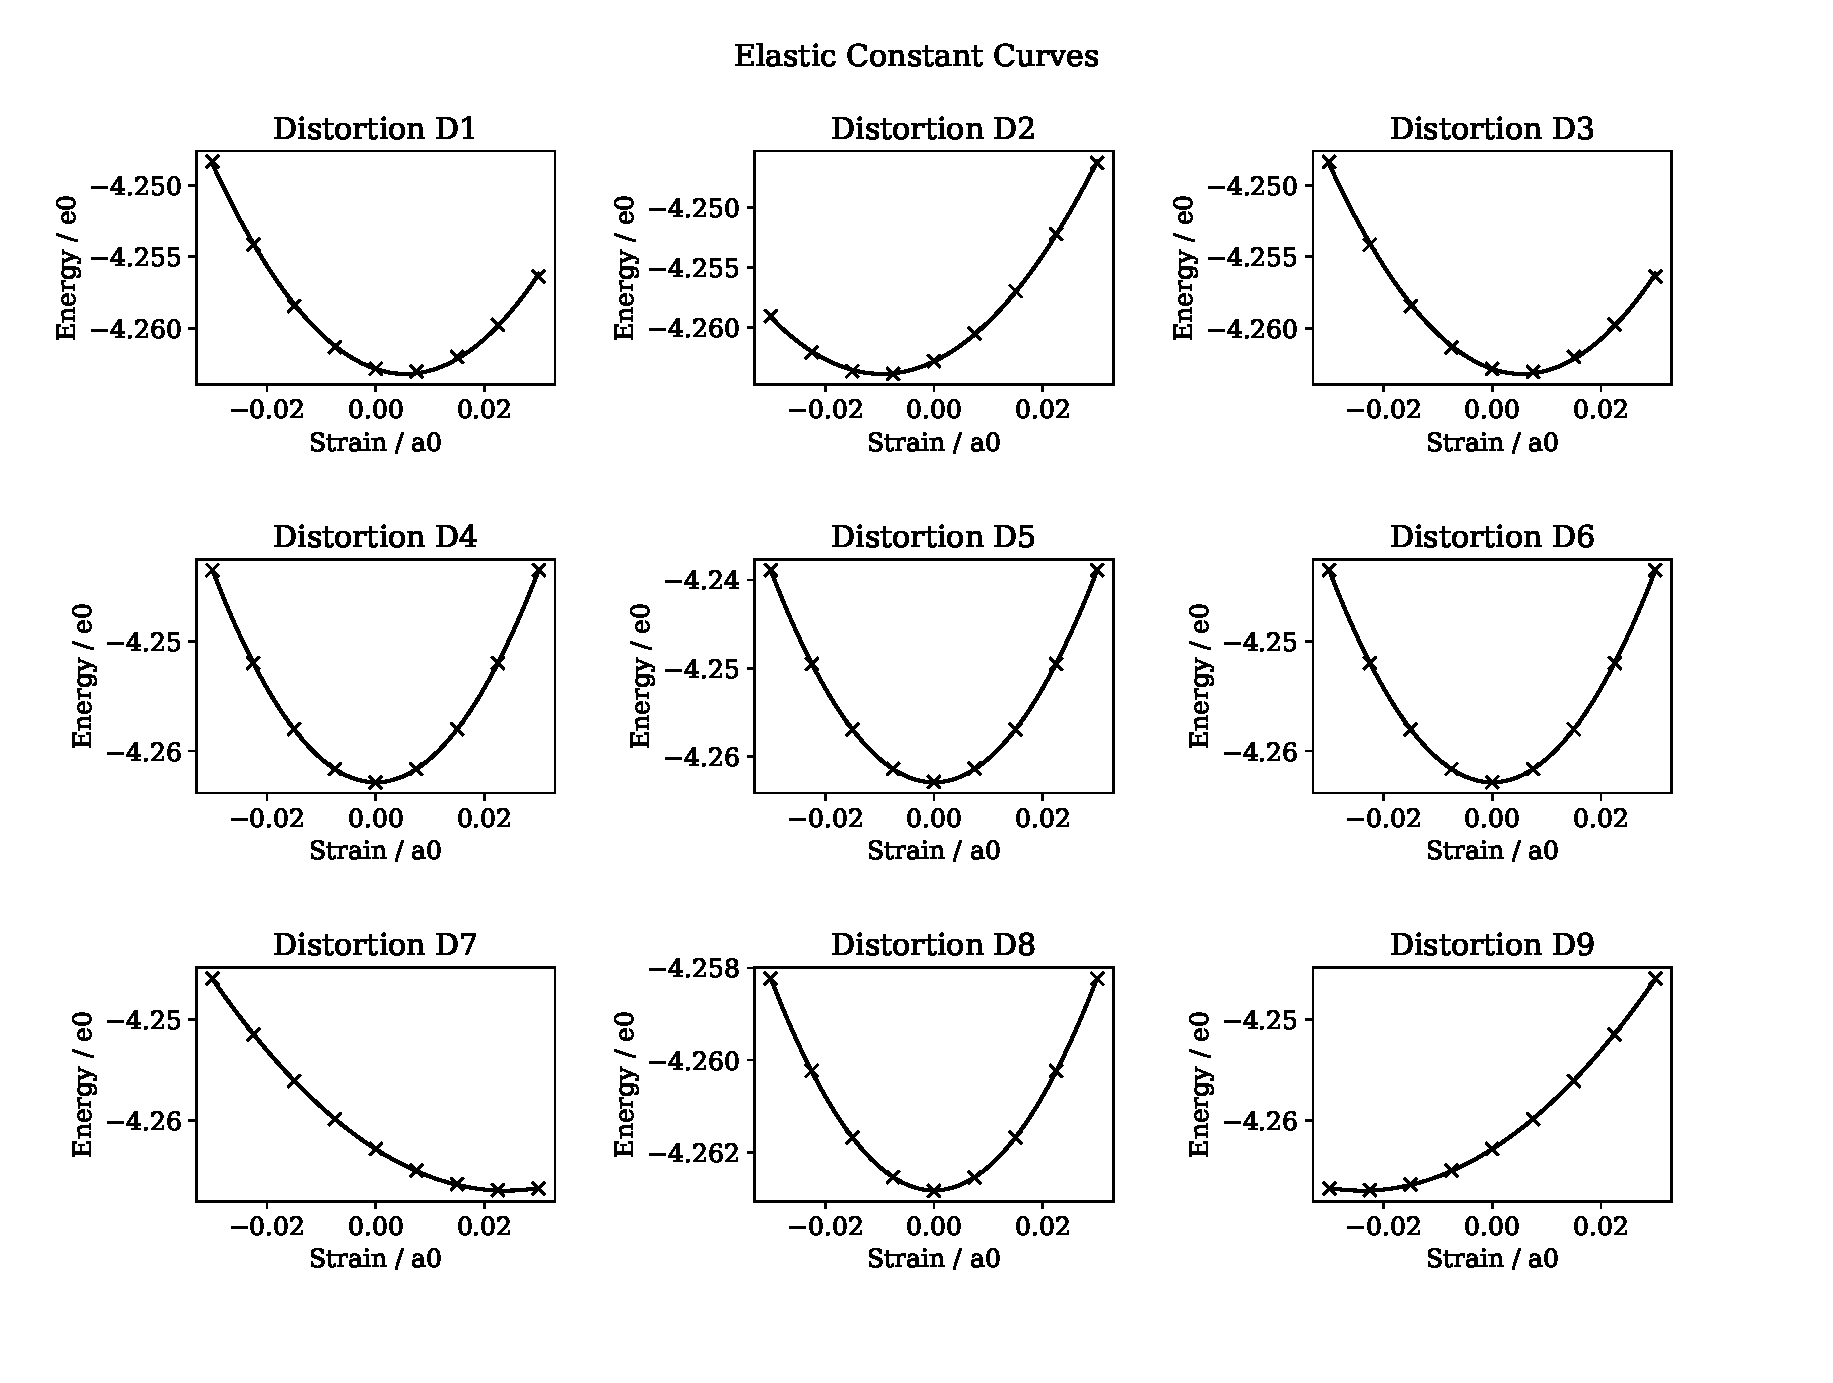
\includegraphics[width=.90\linewidth]{chapters/potentials_fe_pd_ru/feru_potential/ec_rfkj/elastic_strains_bp_1.eps}  
\label{fig:feru-fefcc-distortions}
\caption{Ravindran et al\cite{dftrfkj} distortion-energy plots for \acrshort{fcc} Fe}
\end{figure}

\begin{figure}[htb]
\begin{subfigure}{.42\textwidth}
  \centering
  \includegraphics[width=.90\linewidth]{chapters/potentials_fe_pd_ru/feru_potential/ec_mskp/msp_c11_c12_plot_bp_1.eps}  
  \caption{C11-C12 orthorhombic distortion}
  \label{fig:feru-fefcc-c11c12}
\end{subfigure}
\begin{subfigure}{.42\textwidth}
  \centering
  \includegraphics[width=.90\linewidth]{chapters/potentials_fe_pd_ru/feru_potential/ec_mskp/msp_c44_plot_bp_1.eps}  
  \caption{C44 monoclinic distortion}
  \label{fig:feru-fefcc-c44}
\end{subfigure}
\label{fig:feru-fefcc-c11c12c44}
\caption{\acrshort{mskp} elastic constant strains, where the solid line is the known value and the points the values for this potential - \acrshort{fcc} Fe}
\end{figure}







%%%%%%%%%%%%%%%%%%%%%%%%%%%%%%%%%%%%%%%%%%%%%%%%%%%%%%%%%%%%%%%%%%%%%%
%  Ruthenium FCC Bulk Properties
%%%%%%%%%%%%%%%%%%%%%%%%%%%%%%%%%%%%%%%%%%%%%%%%%%%%%%%%%%%%%%%%%%%%%%

\clearpage
\FloatBarrier
\subsection{Ruthenium FCC}

\begin{table}[ht]
\renewcommand{\arraystretch}{1.2}
\centering
\resizebox{\columnwidth}{!}{%
\begin{tabular}{lcccccc}
\hline\hline
Property & \multicolumn{3}{c}{DFT Computed} & \multicolumn{3}{c}{This Potential} \\
\hline\hline
$a_0$ (angs)         & \multicolumn{3}{c}{3.81}   & \multicolumn{3}{c}{3.79} \\
Basis            & \multicolumn{3}{c}{$\begin{bmatrix} 1.0 & 0.0 & 0.0 \\ 0.0 & 1.0 & 0.0 \\ 0.0 & 0.0 & 1.0  \end{bmatrix}$} & \multicolumn{3}{c}{$\begin{bmatrix} 1.0 & 0.0 & 0.0 \\ 0.0 & 1.0 & 0.0 \\ 0.0 & 0.0 & 1.0  \end{bmatrix}$} \\
$E_{coh}$ (eV)           & \multicolumn{3}{c}{-6.62}  & \multicolumn{3}{c}{-6.61} \\
$B_0$ (GPa)              & \multicolumn{3}{c}{307.8(a) 303.3(b)}  & \multicolumn{3}{c}{331.1(a) 320.4(b)} \\
Stiff.1 (GPa) & \multicolumn{3}{c}{$\begin{bmatrix} 471.5 & 219.1 & 219.2 & 0 & 0 & 0 \\ 219.1 & 471.5 & 219.2 & 0 & 0 & 0 \\ 219.2 & 219.2 & 471.7 & 0 & 0 & 0 \\ 0 & 0 & 0 & 245.0 & 0 & 0 \\ 0 & 0 & 0 & 0 & 245.0 & 0 \\ 0 & 0 & 0 & 0 & 0 & 245.0 \end{bmatrix}$}   & \multicolumn{3}{c}{$\begin{bmatrix} 368.3 & 296.5 & 296.5 & 0 & 0 & 0 \\ 296.5 & 368.3 & 296.5 & 0 & 0 & 0 \\ 296.5 & 296.5 & 368.3 & 0 & 0 & 0 \\ 0 & 0 & 0 & 104.0 & 0 & 0 \\ 0 & 0 & 0 & 0 & 104.0 & 0 \\ 0 & 0 & 0 & 0 & 0 & 104.0 \end{bmatrix}$} \\
Stiff.2 (GPa) & \multicolumn{3}{c}{}   & \multicolumn{3}{c}{$\begin{bmatrix} 375.0 & 309.2 & 309.2 & 0 & 0 & 0 \\ 309.2 & 375.0 & 309.2 & 0 & 0 & 0 \\ 309.2 & 309.2 & 375.0 & 0 & 0 & 0 \\ 0 & 0 & 0 & 97.5 & 0 & 0 \\ 0 & 0 & 0 & 0 & 97.5 & 0 \\ 0 & 0 & 0 & 0 & 0 & 97.5 \end{bmatrix}$} \\
\hline\hline
\end{tabular}%
}
\caption{The lattice parameter, cohesive energy and bulk modulus were determined by fitting the Birch-Murnaghan equation of state.  The bulk modulus is computed from the Birch-Murnaghan equation of state (a) and the average Reuss and Voight Bulk Moduldus (b). The elastic constants computed for the potential in stiffness (1) were computed using the method by Ravindran et al\cite{dfttisiravindran} and in stiffness (2) by Mehl et al\cite{mehlsp}\cite{elasticpropertiesmehl}.}
\end{table}


\subsubsection{Equation of State Plots}

Both the Birch-Murnaghan and Rose-Vinet equation of states are used in the fitting process.

\begin{figure}[htb]
\begin{subfigure}{.44\textwidth}
  \centering
  \includegraphics[width=.94\linewidth]{chapters/potentials_fe_pd_ru/feru_potential/eos/rose_plot_bp_2.eps}  
  \caption{Rose-Vinet}
  \label{fig:feru-fefcc-rose}
\end{subfigure}
\begin{subfigure}{.44\textwidth}
  \centering
  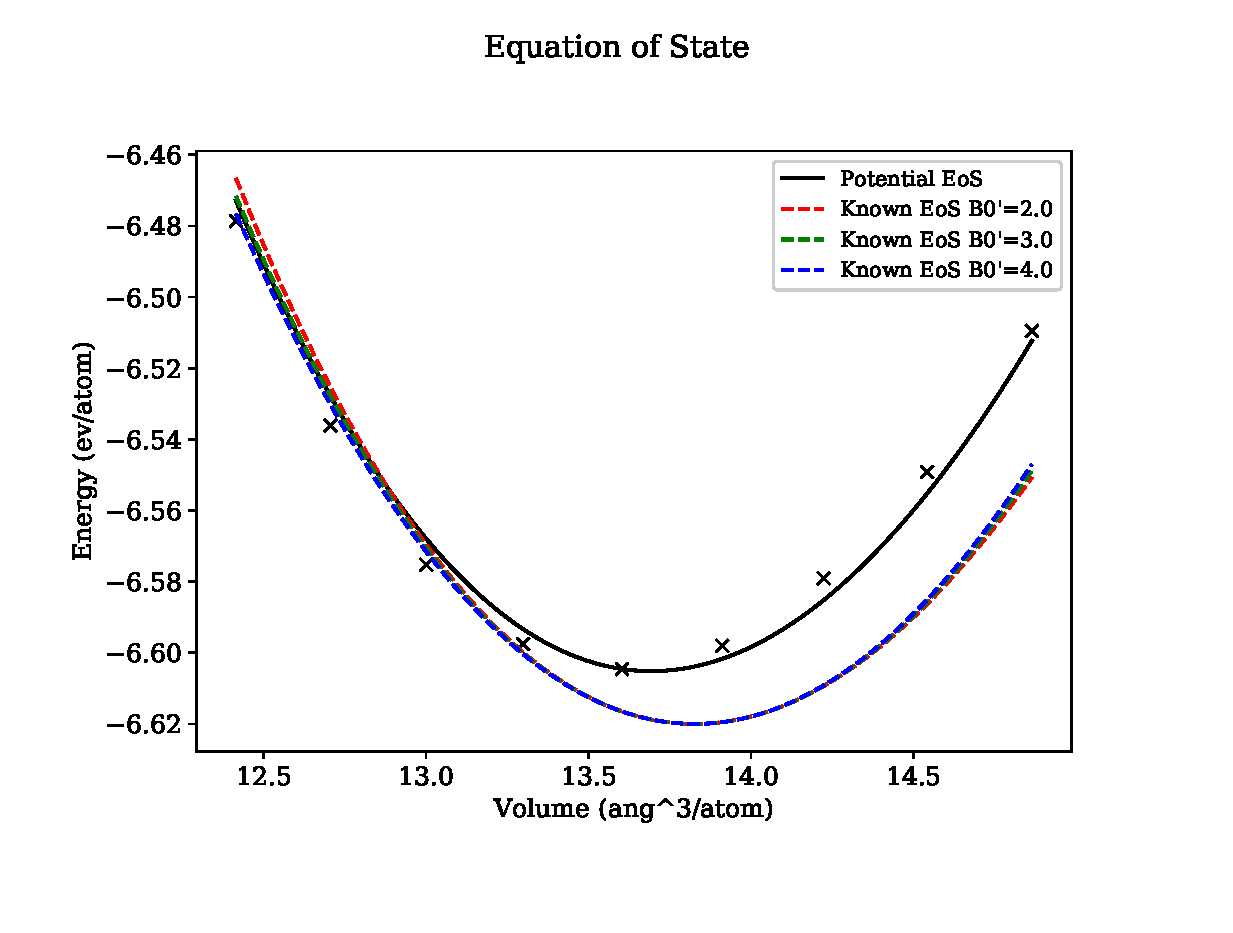
\includegraphics[width=.94\linewidth]{chapters/potentials_fe_pd_ru/feru_potential/eos/equation_of_state_bp_2.eps}  
  \caption{Birch Murnaghan}
  \label{fig:feru-fefcc-bmeos}
\end{subfigure}
\label{fig:feru-fefcc-equation-of-state}
\caption{Equation of State plots from this potential for \acrshort{fcc} Ru}
\end{figure}


\clearpage
\subsubsection{Elastic Constant Plots}

\begin{figure}[htb]
\centering
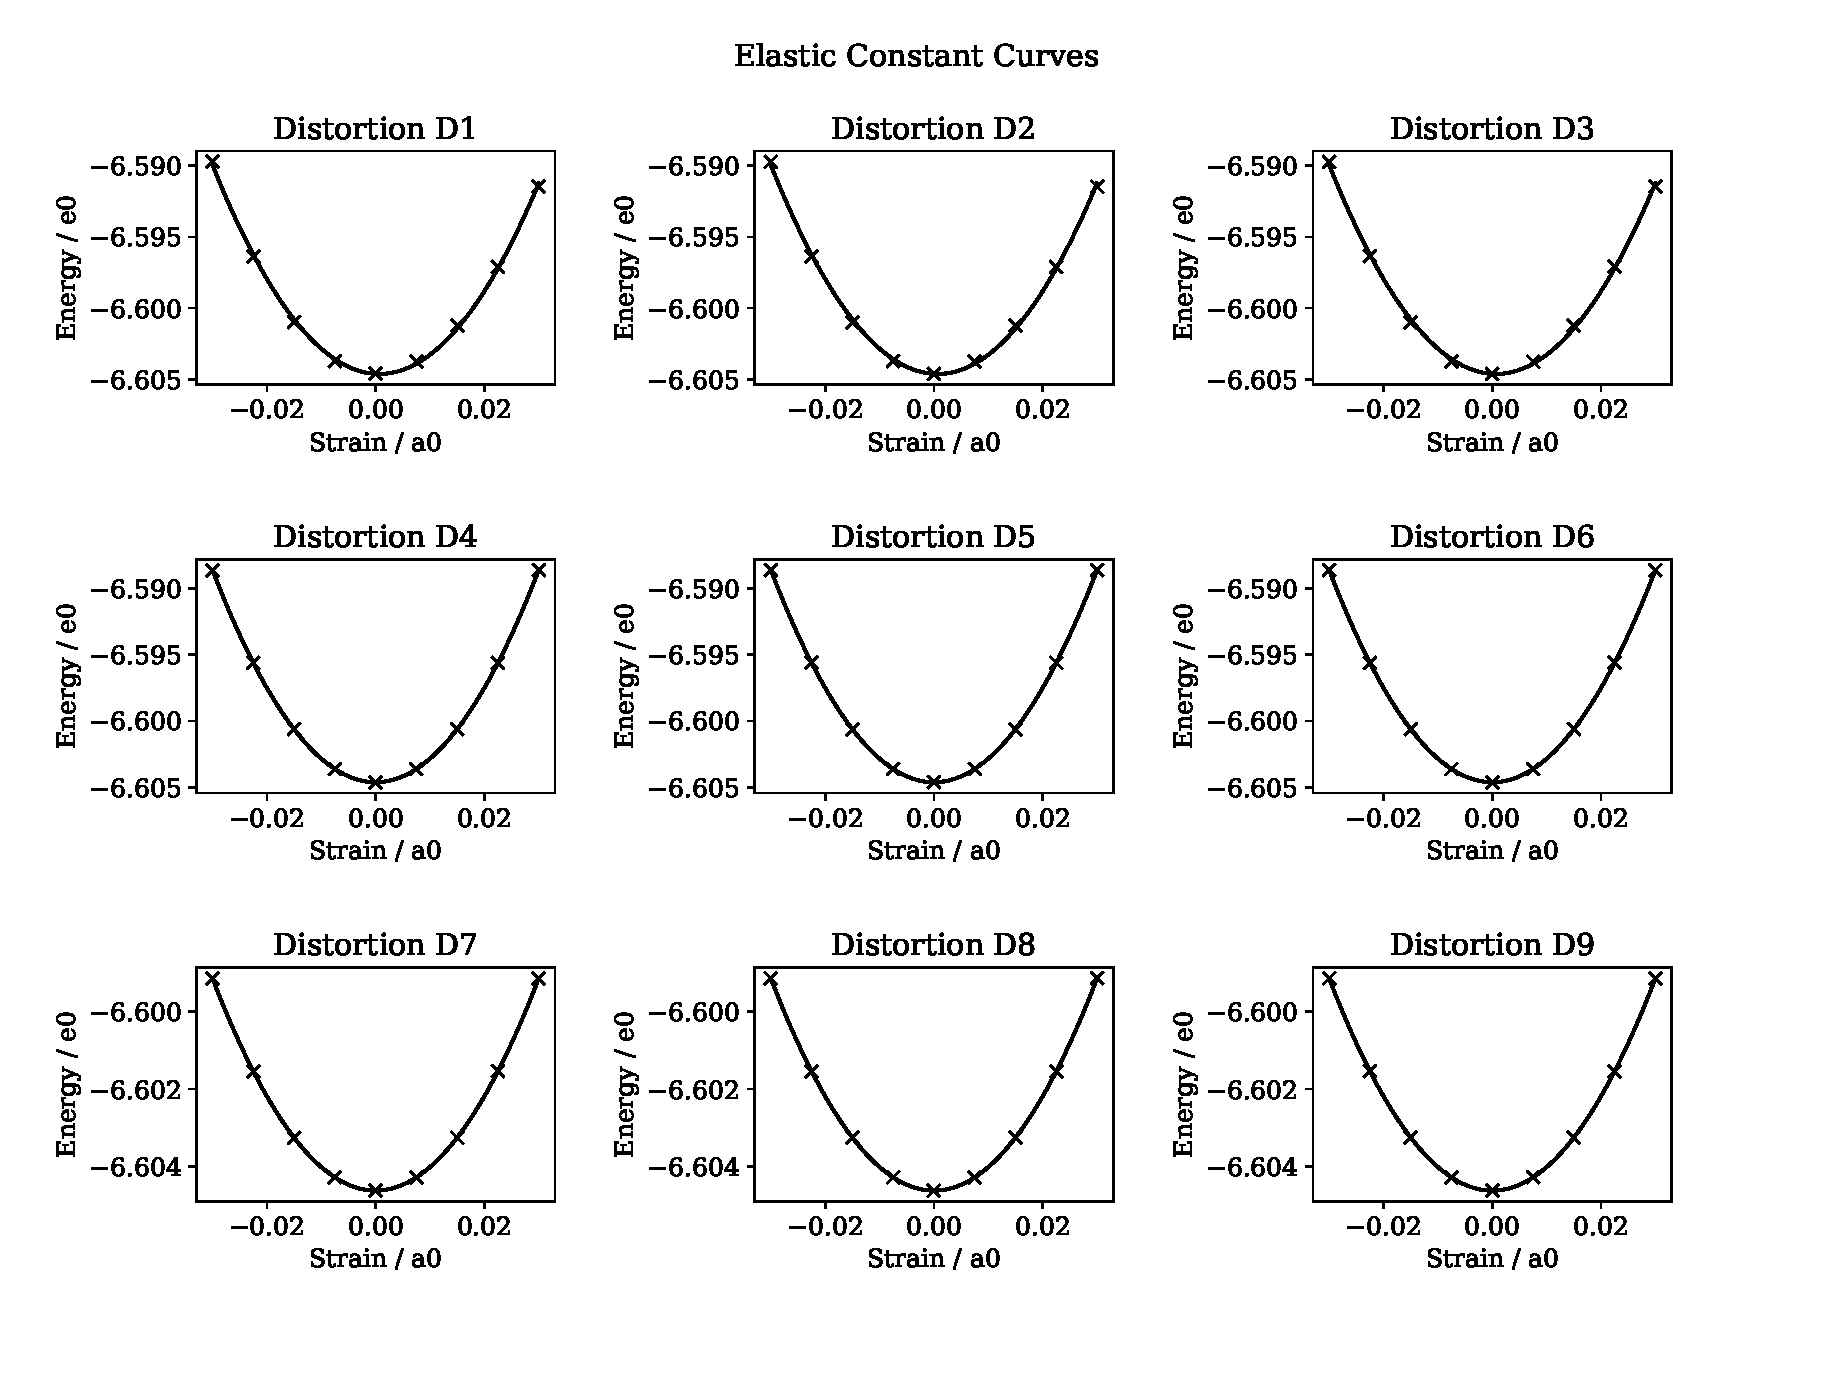
\includegraphics[width=.90\linewidth]{chapters/potentials_fe_pd_ru/feru_potential/ec_rfkj/elastic_strains_bp_2.eps}  
\label{fig:feru-fefcc-rose}
\caption{Ravindran et al\cite{dftrfkj} distortion-energy plots for \acrshort{fcc} Ru}
\end{figure}

\begin{figure}[htb]
\begin{subfigure}{.42\textwidth}
  \centering
  \includegraphics[width=.90\linewidth]{chapters/potentials_fe_pd_ru/feru_potential/ec_mskp/msp_c11_c12_plot_bp_2.eps}  
  \caption{C11-C12 orthorhombic distortion}
  \label{fig:feru-fefcc-c11c12}
\end{subfigure}
\begin{subfigure}{.42\textwidth}
  \centering
  \includegraphics[width=.90\linewidth]{chapters/potentials_fe_pd_ru/feru_potential/ec_mskp/msp_c44_plot_bp_2.eps}  
  \caption{C44 monoclinic distortion}
  \label{fig:feru-fefcc-c11c12c44}
\end{subfigure}
\label{fig:fig:fepd-fefcc-equation-of-state}
\caption{\acrshort{mskp} elastic constant strains, where the solid line is the known value and the points the values for this potential - \acrshort{fcc} Ru}
\end{figure}



%%%%%%%%%%%%%%%%%%%%%%%%%%%%%%%%%%%%%%%%%%%%%%%%%%%%%%%%%%%%%%%%%%%%%%
%  Iron BCC Bulk Properties
%%%%%%%%%%%%%%%%%%%%%%%%%%%%%%%%%%%%%%%%%%%%%%%%%%%%%%%%%%%%%%%%%%%%%%

\clearpage
\FloatBarrier
\subsection{Iron BCC}


\begin{table}[ht]
\renewcommand{\arraystretch}{1.2}
\centering
\resizebox{\columnwidth}{!}{%
\begin{tabular}{lcccccc}
\hline\hline
Property & \multicolumn{3}{c}{DFT Computed} & \multicolumn{3}{c}{This Potential} \\
\hline\hline
$a_0$ (angs)         & \multicolumn{3}{c}{2.80}   & \multicolumn{3}{c}{2.76} \\
Basis            & \multicolumn{3}{c}{$\begin{bmatrix} 1.0 & 0.0 & 0.0 \\ 0.0 & 1.0 & 0.0 \\ 0.0 & 0.0 & 1.0  \end{bmatrix}$} & \multicolumn{3}{c}{$\begin{bmatrix} 1.0 & 0.0 & 0.0 \\ 0.0 & 1.0 & 0.0 \\ 0.0 & 0.0 & 1.0  \end{bmatrix}$} \\
$E_{coh}$ (eV)           & \multicolumn{3}{c}{-4.32}  & \multicolumn{3}{c}{-4.16} \\
$B_0$ (GPa)              & \multicolumn{3}{c}{239.2(a) 205.3(b)}  & \multicolumn{3}{c}{229.0(a) 207.6(b)} \\
Stiff.1 (GPa) & \multicolumn{3}{c}{$\begin{bmatrix} 250.1 & 182.3 & 183.3 & 0 & 0 & 0 \\ 182.3 & 249.1 & 182.9 & 0 & 0 & 0 \\ 183.2 & 182.9 & 251.2 & 0 & 0 & 0 \\ 0 & 0 & 0 & 139.2 & 0 & 0 \\ 0 & 0 & 0 & 0 & 139.7 & 0 \\ 0 & 0 & 0 & 0 & 0 & 139.3 \end{bmatrix}$}   & \multicolumn{3}{c}{$\begin{bmatrix} 178.8 & 222.0 & 222.0 & 0 & 0 & 0 \\ 222.0 & 178.8 & 222.0 & 0 & 0 & 0 \\ 222.0 & 222.0 & 178.8 & 0 & 0 & 0 \\ 0 & 0 & 0 & 215.2 & 0 & 0 \\ 0 & 0 & 0 & 0 & 215.2 & 0 \\ 0 & 0 & 0 & 0 & 0 & 215.2 \end{bmatrix}$} \\
Stiff.2 (GPa) & \multicolumn{3}{c}{}   & \multicolumn{3}{c}{$\begin{bmatrix} 190.1 & 248.5 & 248.5 & 0 & 0 & 0 \\ 248.5 & 190.1 & 248.5 & 0 & 0 & 0 \\ 248.5 & 248.5 & 190.1 & 0 & 0 & 0 \\ 0 & 0 & 0 & 168.7 & 0 & 0 \\ 0 & 0 & 0 & 0 & 168.7 & 0 \\ 0 & 0 & 0 & 0 & 0 & 168.7 \end{bmatrix}$} \\
\hline\hline
\end{tabular}%
}
\caption{The lattice parameter, cohesive energy and bulk modulus were determined by fitting the Birch-Murnaghan equation of state.  The bulk modulus is computed from the Birch-Murnaghan equation of state (a) and the average Reuss and Voight Bulk Moduldus (b). The elastic constants computed for the potential in stiffness (1) were computed using the method by Ravindran et al\cite{dfttisiravindran} and in stiffness (2) by Mehl et al\cite{mehlsp}\cite{elasticpropertiesmehl}.}
\end{table}



\subsubsection{Equation of State Plots}

Both the Birch-Murnaghan and Rose-Vinet equation of states are used in the fitting process.

\begin{figure}[htb]
\begin{subfigure}{.44\textwidth}
  \centering
  \includegraphics[width=.94\linewidth]{chapters/potentials_fe_pd_ru/feru_potential/eos/rose_plot_bp_0.eps}  
  \caption{Rose-Vinet}
  \label{fig:feru-febcc-rose}
\end{subfigure}
\begin{subfigure}{.44\textwidth}
  \centering
  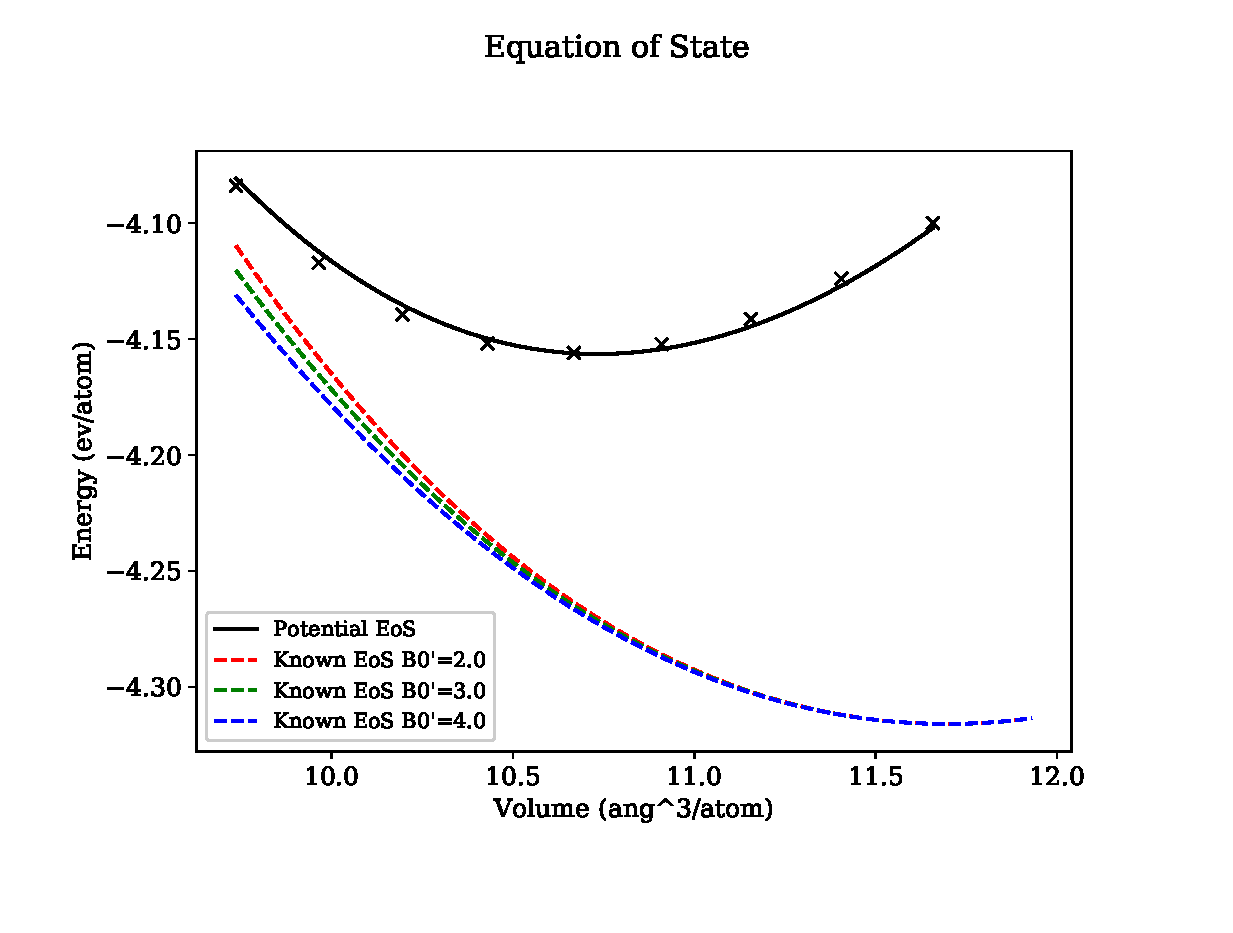
\includegraphics[width=.94\linewidth]{chapters/potentials_fe_pd_ru/feru_potential/eos/equation_of_state_bp_0.eps}  
  \caption{Birch Murnaghan}
  \label{fig:feru-febcc-bmeos}
\end{subfigure}
\label{fig:fepd-febcc-equation-of-state}
\caption{Equation of State plots from this potential for \acrshort{bcc} Fe}
\end{figure}


\clearpage
\subsubsection{Elastic Constant Plots}

\begin{figure}[htb]
\centering
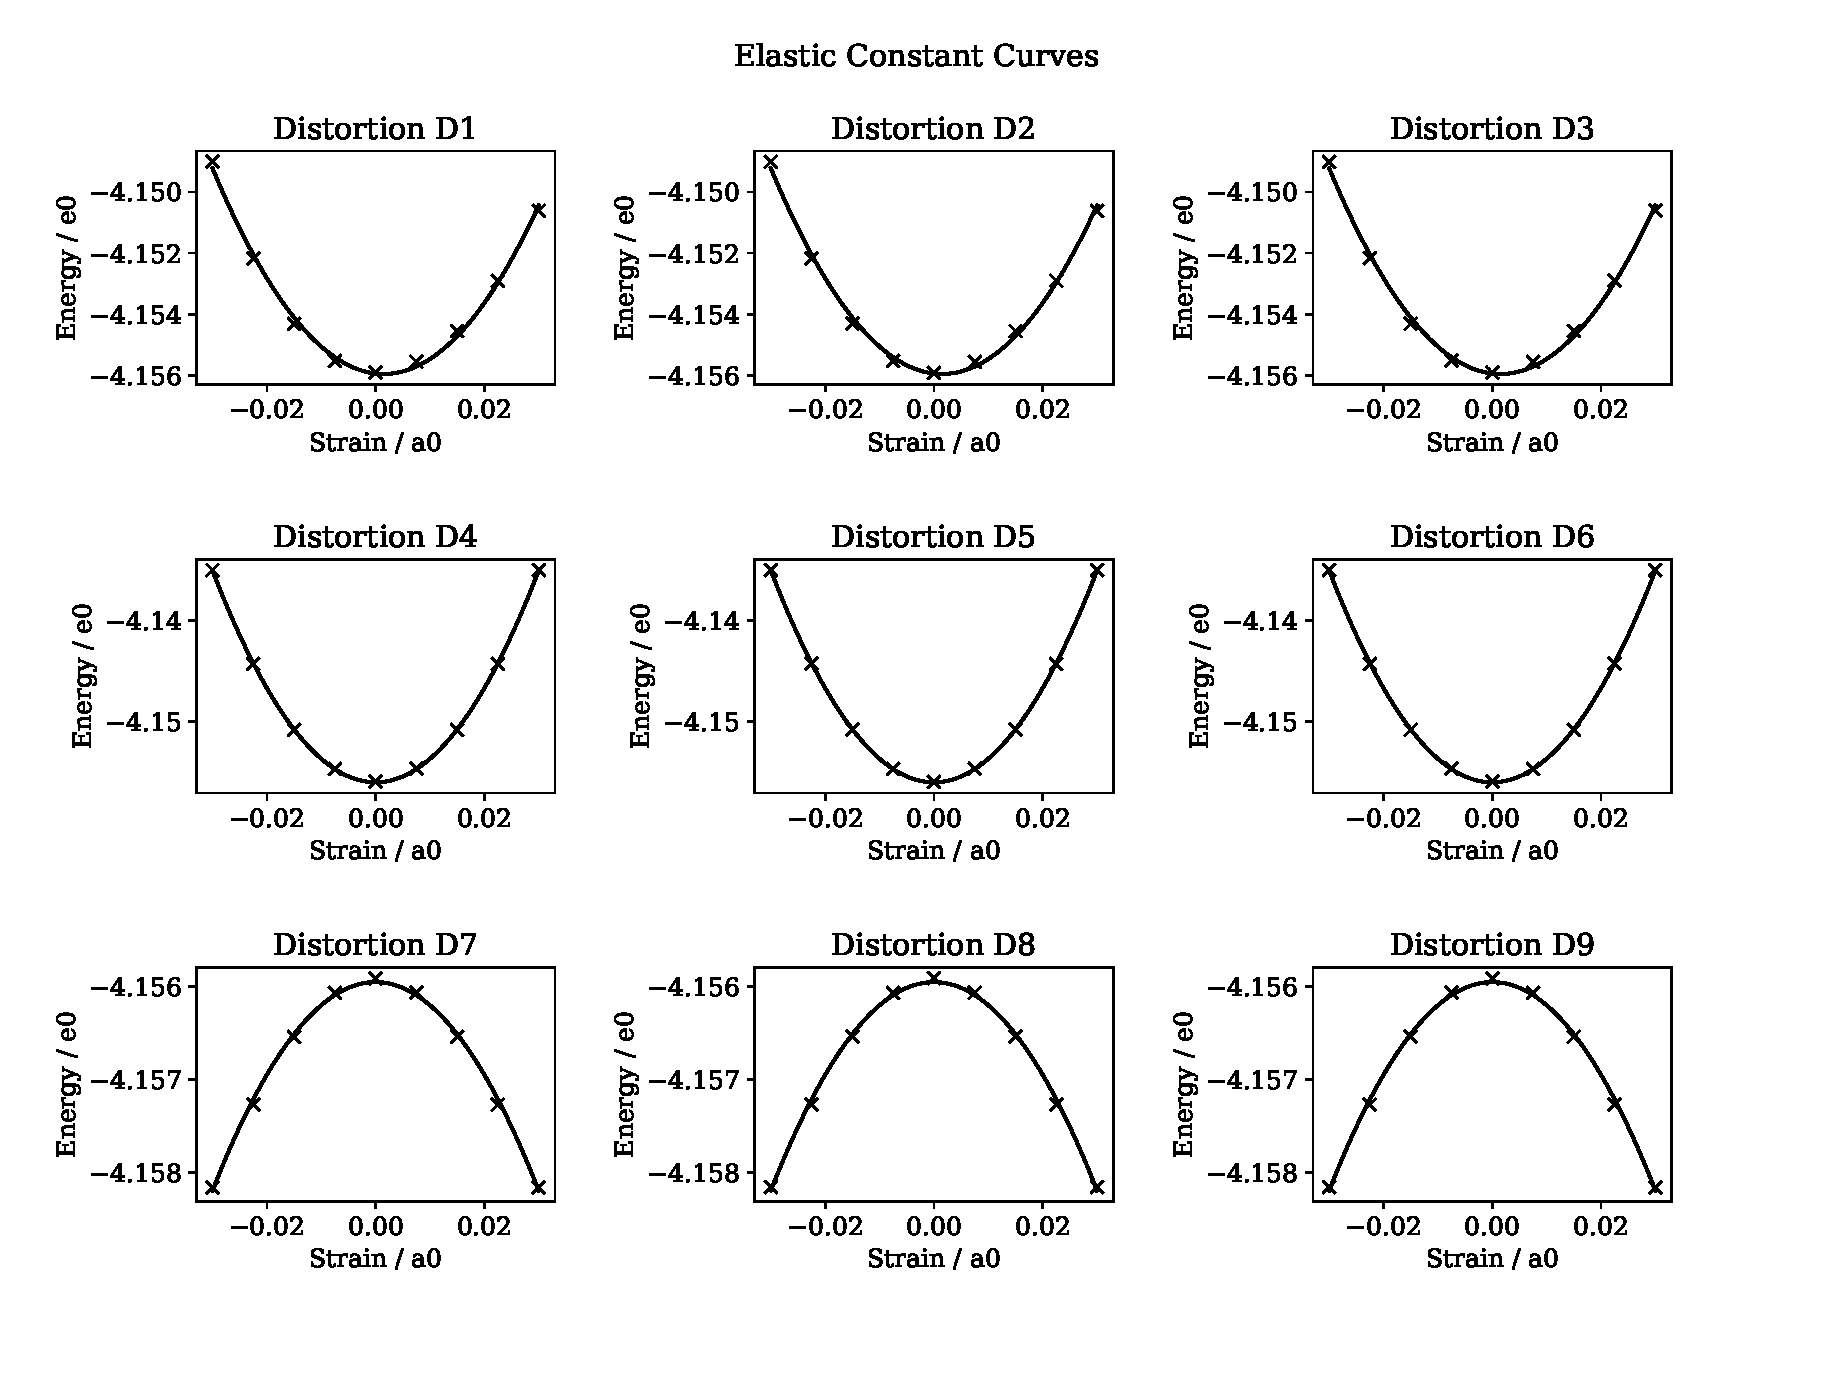
\includegraphics[width=.90\linewidth]{chapters/potentials_fe_pd_ru/feru_potential/ec_rfkj/elastic_strains_bp_0.eps}  
\label{fig:feru-rufcc-rose}
\caption{Ravindran et al\cite{dftrfkj} distortion-energy plots for \acrshort{fcc} Ru}
\end{figure}

\begin{figure}[htb]
\begin{subfigure}{.42\textwidth}
  \centering
  \includegraphics[width=.90\linewidth]{chapters/potentials_fe_pd_ru/feru_potential/ec_mskp/msp_c11_c12_plot_bp_0.eps}  
  \caption{C11-C12 orthorhombic distortion}
  \label{fig:fepd-fefcc-rose}
\end{subfigure}
\begin{subfigure}{.42\textwidth}
  \centering
  \includegraphics[width=.90\linewidth]{chapters/potentials_fe_pd_ru/feru_potential/ec_mskp/msp_c44_plot_bp_0.eps}  
  \caption{C44 monoclinic distortion}
  \label{fig:fepd-fefcc-bmeos}
\end{subfigure}
\label{fig:fefcc-equation-of-state}
\caption{\acrshort{mskp} elastic constant strains, where the solid line is the known value and the points the values for this potential - \acrshort{bcc} Ru}
\end{figure}







